\section{Discussion}
\label{sec:discussion}

This thesis arises from a series of problems identified in 2010, when Imhotep
was developed as a response to the observed demand of adaptive user interfaces 
solutions for people with disabilities. Dealing with the available technology
and analysed approaches a solution in which developers were given an \ac{api}
for developing adaptive interfaces was designed. Based on preprocessor primitives,
developers were able to include pieces of source code in which user interface
configuration were completed with a user and a device profile. Those profiles
were given by the potential users through another application.

Imhotep was highly accepted by the scientific community. Several publications
were produced (as shown in Section~\ref{sec:publications}) and an award was 
given based on the AssistedCity developed use case.

However, in spite of the success of Imhotep, technology improvements regarding
mobile devices bring new challenges and possibilities. Thus, from the weaknesses
of Imhotep new solutions arose. These challenges were which conceived AdaptUI.

First, a further analysis of the literature and state of the art in user 
interface adaptation solutions was needed. The lack of mobile based user 
interface adaptive solutions was identified. Besides, the current ongoing 
software and hardware mobile devices improvements enhanced the design of a 
mobile platform.

After taking the decision of using a mobile centred platform, the challenge of
what and how to model arose. Based on our previous experience and on the reviewed
literature a semantic model based on three entities was conceived. This model
mainly combines user's interaction characteristics, a current context situation
description, and different device's characteristics. As one of the identified
problems in the analysed user adaptation platforms in the literature is their
lack of independence from the considered domain, a semantic based design determined.
This allows an easy method to represent the knowledge of the domain, extend it,
share it, and adapt it to any desired sub-domain by just combining different 
ontologies with the provided AdaptUIOnt.

The combination of the two previous mentioned decisions brought a significant
problem: the lack of available mobile based semantic reasoning engines. Therefore,
as a technical contribution AdaptUI provides a mobile reasoning engine based on
Pellet and compatible with Android. It is called \textit{Pellet4Android}, it is
open source, and it provides support for \ac{owl} 2 and \ac{swrl} rules in Android.

Once the semantic models and the mobile semantic infrastructure for reasoning
were operative, the required architecture was design, as is shown in Figure~\ref{fig:architecture_discussion}.

\begin{figure}[H]
\centering
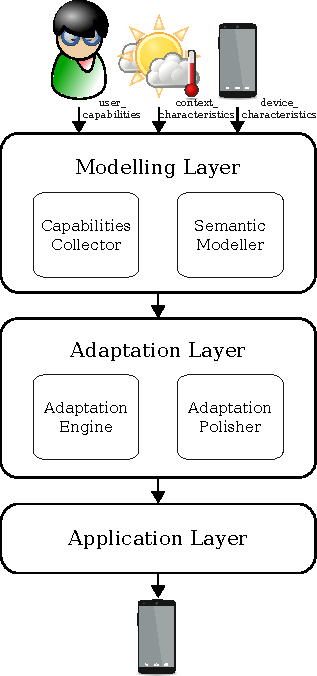
\includegraphics[width=0.30\textwidth]{architecture.pdf}
\caption{AdaptUI's three-layered global architecture.}
\label{fig:architecture_discussion}
\end{figure}

Besides, in order to make AdaptUI accessible for developers, two main \acp{api}
are provided. These \acp{api} aim to allow developers not only to adapt the
user interfaces of their application, but also to adapt the whole AdaptUI platform
to the domain they work with.

% In this thesis several contributions have been provided: First, in 
% Chapter~\ref{cha:ontology_model}, the AdaptUIOnt ontology has been presented. 
% AdaptUIOnt is an ontology that models user interaction capabilities, context 
% current situation and device characteristics with a design that allows a dynamic 
% update of the represented knowledge. Second, \textit{Pellet4android} has been
% introduced in Chapter~\ref{cha:architecture}. \textit{Pellet4android} is a 
% semantic reasoning engine based on Pellet but compatible with Android devices.
% Finally, AdaptUI, a whole dynamic user interface adaptation platform, which 
% allows developers to design adaptive user interfaces for their applications, has 
% been described.

% As AdaptUIOnt has been first highlighted, in the following lines we summarize 
% several conclusions and benefits of the cited designed ontology:
% In the following lines we summarize several conclusions and benefits of AdaptUIOnt:
% 
% \begin{itemize}
%   \item AdaptUIOnt arises from the identified weaknesses of the models and solutions
%   reviewed in Chapter~\ref{cha:state_of_the_art}. Centred on the user needs, it
%   models several characteristics that define users, context and devices, 
%   regarding the current needs for the interaction with the current user 
%   interface, and allowing their semantic representation. 
% 
%   \item AdaptUIOnt allows the modelling of non physiological interaction 
%   capabilities of the user. As mentioned in Chapter~\ref{cha:state_of_the_art}, 
%   several solutions aiming the adaptation of user interfaces (or services) 
%   take into account user physiological capabilities. However, these solutions 
%   assume that these capabilities are properly provided by the user or by 
%   external services. But the truth is that, analysing these solutions, no 
%   experts are consulted or included in the researches. Thus, to us these 
%   solutions, although they are interesting, do not cover the reality of the 
%   users and their daily limitations when dealing with interaction activities. 
%   Hence, the AdaptUIOnt ontology has been designed taking into account this 
%   issue. By avoiding the inclusion of physiological knowledge about user's 
%   capabilities we allow users to directly manipulate their applications without 
%   considering specific expertise or medical background. Besides, developers do 
%   not have to consult any expert in the area, as the translation of the user 
%   interactions are represented in the ontology as preferences and needs, not as 
%   capabilities.
% 
%   \item It allows the addition of external ontologies to complete the knowledge 
%   of the main entities. One of the benefits of semantic representation is the
%   ability to join external ontologies which can enrich the knowledge base. Thus,
%   developers are allowed to design their models or use those ontologies they
%   prefer to better fit AdaptUI in their domains. For example, \textit{Context}
%   has not been designed from scratch. Several extra ontologies, fully supported
%   and used by the community, have been used to build the corresponding knowledge
%   about the context. 
% \end{itemize}
% 
% As the AdaptUI platform is based on semantics and reasoning, a mobile reasoning 
% engine is required. The ported \textit{Pellet4Android} reasoning engine provides
% several benefits, all inherited from Pellet for Java. Although, as is remarked
% in Chapter~\ref{cha:evaluation}, more tests are needed to assure a similar
% performance in mobile devices. Nevertheless, this port provides:
% 
% \begin{itemize}
%   \item Representation and reasoning about information using \ac{owl} in Android
%   based mobile devices.
%   
%   \item Support for \ac{owl} 2 for Android devices.
%   
% %   \item 
% \end{itemize}
% 
% Finally, regarding the whole AdaptUI platform:
% 
% \begin{itemize}
%   \item It allows users to configure the best suitable adaptation regarding their 
%   capabilities, temporary disabilities, context current characteristics and
%   their devices' dynamic and static set of characteristics. Through a simple
%   application they are able to configure the best user interface combination
%   of components for each case. These configurations are stored in the ontology,
%   indexed by the context disabilities extracted from the reasoning process. 
%   Thus, each time AdaptUI detects a known context situation and reasons over 
%   it. If the same disabilities are sensed, they corresponding user interface 
%   is adapted.
%   
%   \item It also allows developers to forget about the aspect of their applications, regarding
%   inclusive design and adaptation, as the platform automatically manages it. 
%   Besides, they are allowed to modify the knowledge through the provided 
%   \acp{api}. Classes, properties, individuals and rules are fully modifiable, 
%   which gives total liberty to developers to adapt the whole platform to their 
%   needs.
%   
%   \item It provides a fully 100\% mobile adaptation platform. It does not require external
%   processing aid, nor even Internet connectivity. Due to the 
%   \textit{Pellet4Android} reasoning engine every reasoning and semantics
%   management process runs in the mobile. This fact avoids possible failures due
%   to connectivity or network losses.
% \end{itemize}

Although AdaptUI has several benefits and it contributes with the mentioned 
completed goals, the presented platform has also several constraints:

\begin{itemize}
  \item Depending on the hardware of the used devices might lead into 
  performance penalization if such devices have not the necessary computing
  capabilities. Although the results presented in 
  Chapter~\ref{cha:evaluation} brought promising references regarding device's 
  processing capabilities, the less powered device is a Samsung Galaxy SIII Mini.
  
  \item Although we have demonstrated that several temporary context 
  disabilities and limitations are considerably reduced, people with 
  disabilities might still suffer several interaction problems. Thus, further 
  efforts are needed to improve and finalise the whole system. This issue is 
  described in Section~\ref{sec:future_work}.
  
  \item Another limitation is that AdaptUI mostly considers disabilities based
  on visual and hearing constraints. Although others have been studied (as motor
  disabilities), the experiments are difficult to carry out. This is also 
  detailed in Section~\ref{sec:future_work}, as we aim to cover more limitations 
  and experiment with such contexts.
\end{itemize}